\documentclass[16pt]{beamer}
\usepackage[utf8]{inputenc}

\title{Le coût du gratuit}

\usetheme{default}

\usepackage[utf8]{inputenc}
\usepackage{amsmath}
\usepackage{amsfonts}
\usepackage{amssymb}
\usepackage{pgf}
\usepackage{color}
\usepackage[frenchb]{babel}
\usepackage{amssymb}
\usepackage{hyperref}

\usefonttheme{default}
\usepackage{DejaVuSans}
%\usepackage[sfdefault]{FiraSans} %% option 'sfdefault' activates Fira Sans as the default text font
\usepackage[T1]{fontenc}
\renewcommand*\oldstylenums[1]{{\firaoldstyle #1}}


\setbeamertemplate{navigation symbols}{} %remove navigation symbols

\author{Cédric Jeanneret (aka \href{https://www.twitter.com/SwissTengu}{@SwissTengu})}
\institute{\href{https://www.ethack.org/}{EthACK.org}}
\date{\today}

\definecolor{linecolor}{HTML}{4d4c4c}

\setbeamercolor{linecolor}{fg=white,bg=linecolor}

\setbeamertemplate{headline} {
	\begin{beamercolorbox}[wd=\paperwidth,dp=8pt,ht=12pt,leftskip=.29cm,rightskip=.29cm]{linecolor}
	\hfill
	\hypersetup{
		colorlinks=true,
		linkcolor=white,
		urlcolor=white,
	}
	\insertinstitute
	\end{beamercolorbox}%
}

\setbeamertemplate{footline}{%
	\begin{beamercolorbox}[wd=\paperwidth,dp=9pt,ht=0.4cm,leftskip=.29cm,rightskip=.3cm]{linecolor}
	\pgfputat{\pgfxy(0.455,-0.315)}{\pgfbox[center,base]{
\includegraphics[width=1.5cm]{../common/logo_537.png}}}
	\hfill
	\inserttitle
	\end{beamercolorbox}%
}


\hypersetup{
	colorlinks=true,
	linkcolor=blue,
	urlcolor=blue,
	pdfborderstyle={/S/U/W 1},
	pdfborder=0 0 1,
	linkbordercolor={0 0 0},
	urlbordercolor={0 0 0},
}


\begin{document}

{
\setbeamertemplate{footline}{%
	\begin{beamercolorbox}[wd=\paperwidth,dp=8pt,ht=12pt,leftskip=.29cm,rightskip=.3cm]{linecolor}
	\hfill
	\inserttitle
	\end{beamercolorbox}%
}

% center first slide — not a title, but almost
{
\centering
\begin{frame}

EthACK
\vspace{0.5cm}

The Swiss Privacy Basecamp 
\vspace{0.5cm}


\includegraphics[width=4cm]{../common/logo_537.png}

\end{frame}
}
}

\begin{frame}{EthACK ?}
\begin{itemize}
	\item Éthique
	\item État
	\item ACKnowledgement (reconnaissance)
	\item Hacking (éthique, évidemment)
	\item …
\end{itemize}
\end{frame}

\begin{frame}{Pourquoi ?}
\begin{itemize}
	\item Notre gouvernement ne s'intéresse pas (ou peu) au sujet
	\item Les sociétés privées nous fichent à notre insu
	\item Personne ne sait où sont leurs données, qui les traitent, à quoi elles servent
\end{itemize}
\end{frame}


\begin{frame}
  \titlepage
\end{frame}

\begin{frame}
{Plan rapide}
\begin{itemize}
\item Le gratuit
\item L'Opensource
\item Alternatives
\item Exemple comparatif
\item Questions
\end{itemize}
\end{frame}

\begin{frame}
{Viendez c'est gratuit !}
\begin{itemize}
\item "Cloud"
\item Services de synchronisation
\item Partage de fichiers
\item Services Mail
\item Services de messageries
\item …
\end{itemize}
\end{frame}

\begin{frame}
{Tout à un coût}
\begin{itemize}
\item Infrastructure serveur
\item Développeurs
\item Marketting
\item …
\end{itemize}
\end{frame}

\begin{frame}
{Gratuit, coût… ?!}
\centering

\includegraphics[height=4cm,keepaspectratio]{./money-question-mark.jpg}
\end{frame}

\begin{frame}
{Sources}
\begin{itemize}
\item Publicités (intégrées)
\item "Freemium"
\item …
\end{itemize}
\end{frame}

\begin{frame}
{}
\centering
Et, surtout, vos données !
\end{frame}

{
\hypersetup{
        colorlinks=true,
        linkcolor=white,
        urlcolor=white
}
\setbeamertemplate{headline} {
        \begin{beamercolorbox}[wd=\paperwidth,dp=8pt,ht=12pt,leftskip=.29cm,rightskip=.29cm]{linecolor}
        Source: \textbf{\href{https://www.facebook.com/business/}{Facebook}}
        \hfill
        \insertinstitute
        \end{beamercolorbox}%
}
\begin{frame}
\centering
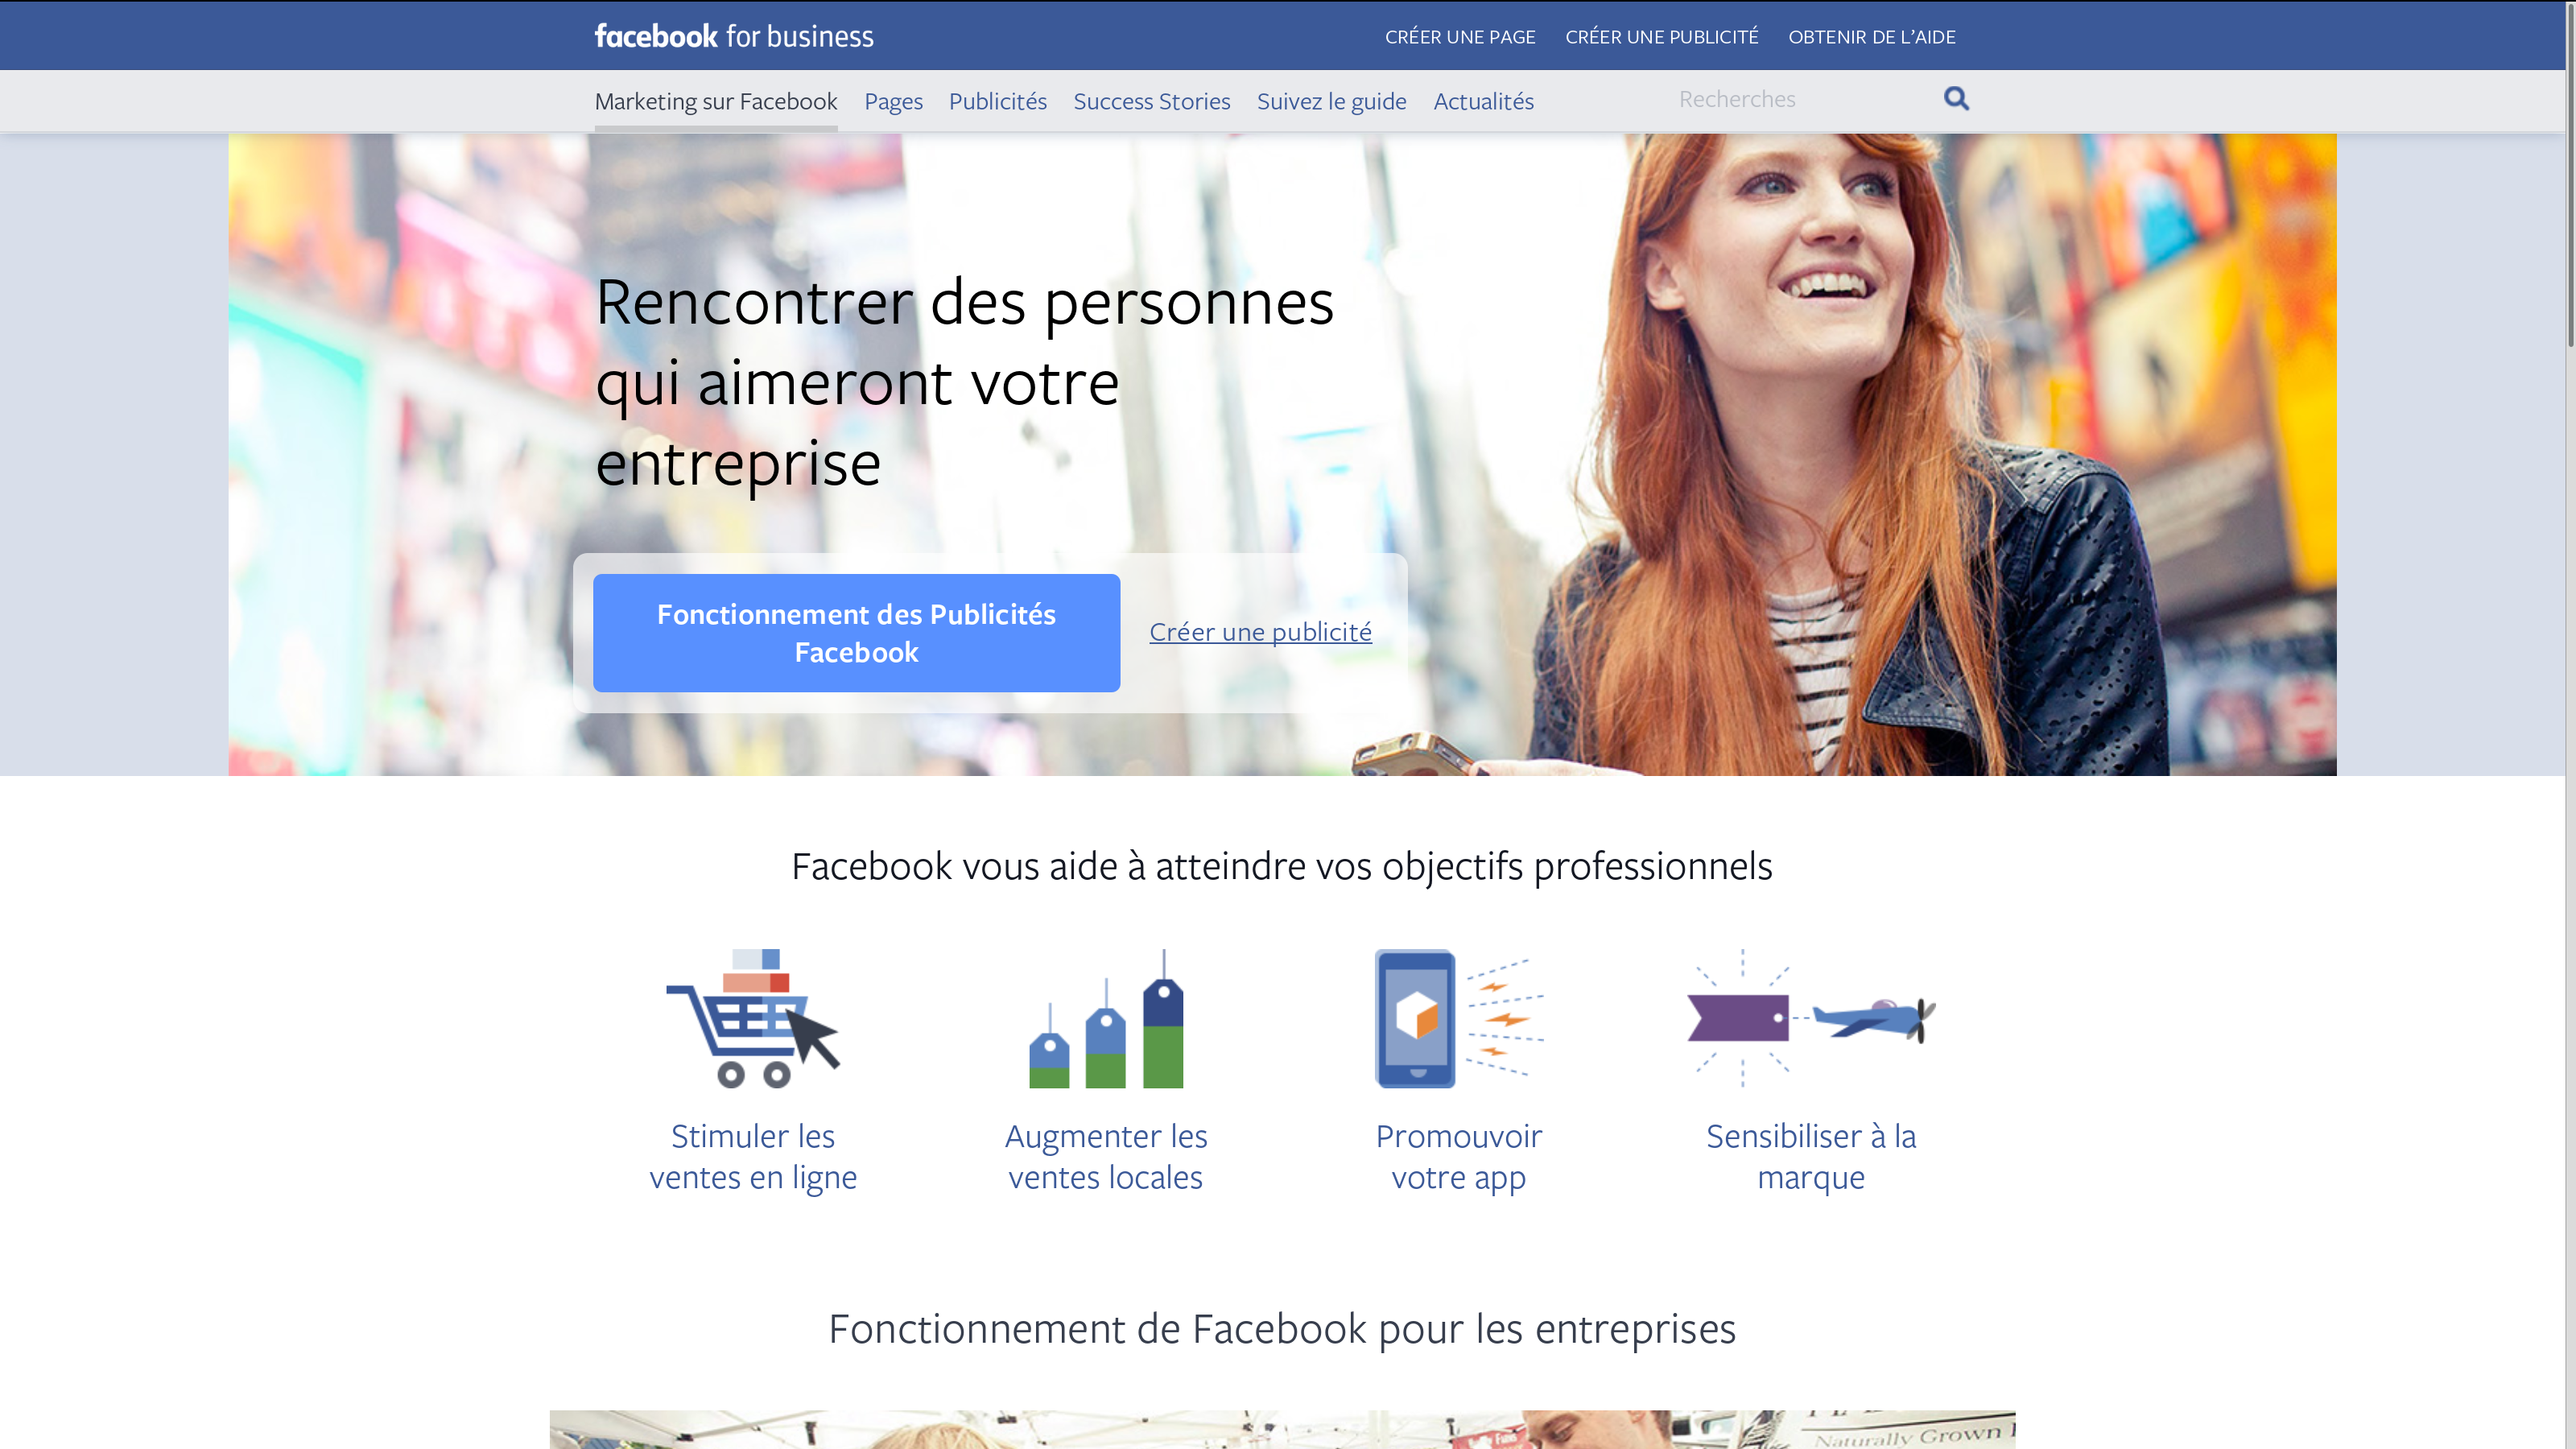
\includegraphics[width=\textwidth,height=\textheight,keepaspectratio]{./facebook.png} 
\end{frame}
}

{
\hypersetup{
        colorlinks=true,
        linkcolor=white,
        urlcolor=white
}
\setbeamertemplate{headline} {
        \begin{beamercolorbox}[wd=\paperwidth,dp=8pt,ht=12pt,leftskip=.29cm,rightskip=.29cm]{linecolor}
        Source: \textbf{\href{https://www.google.fr/adwords/?zd=1}{Google}}
        \hfill
        \insertinstitute
        \end{beamercolorbox}%
}
\begin{frame}
\centering
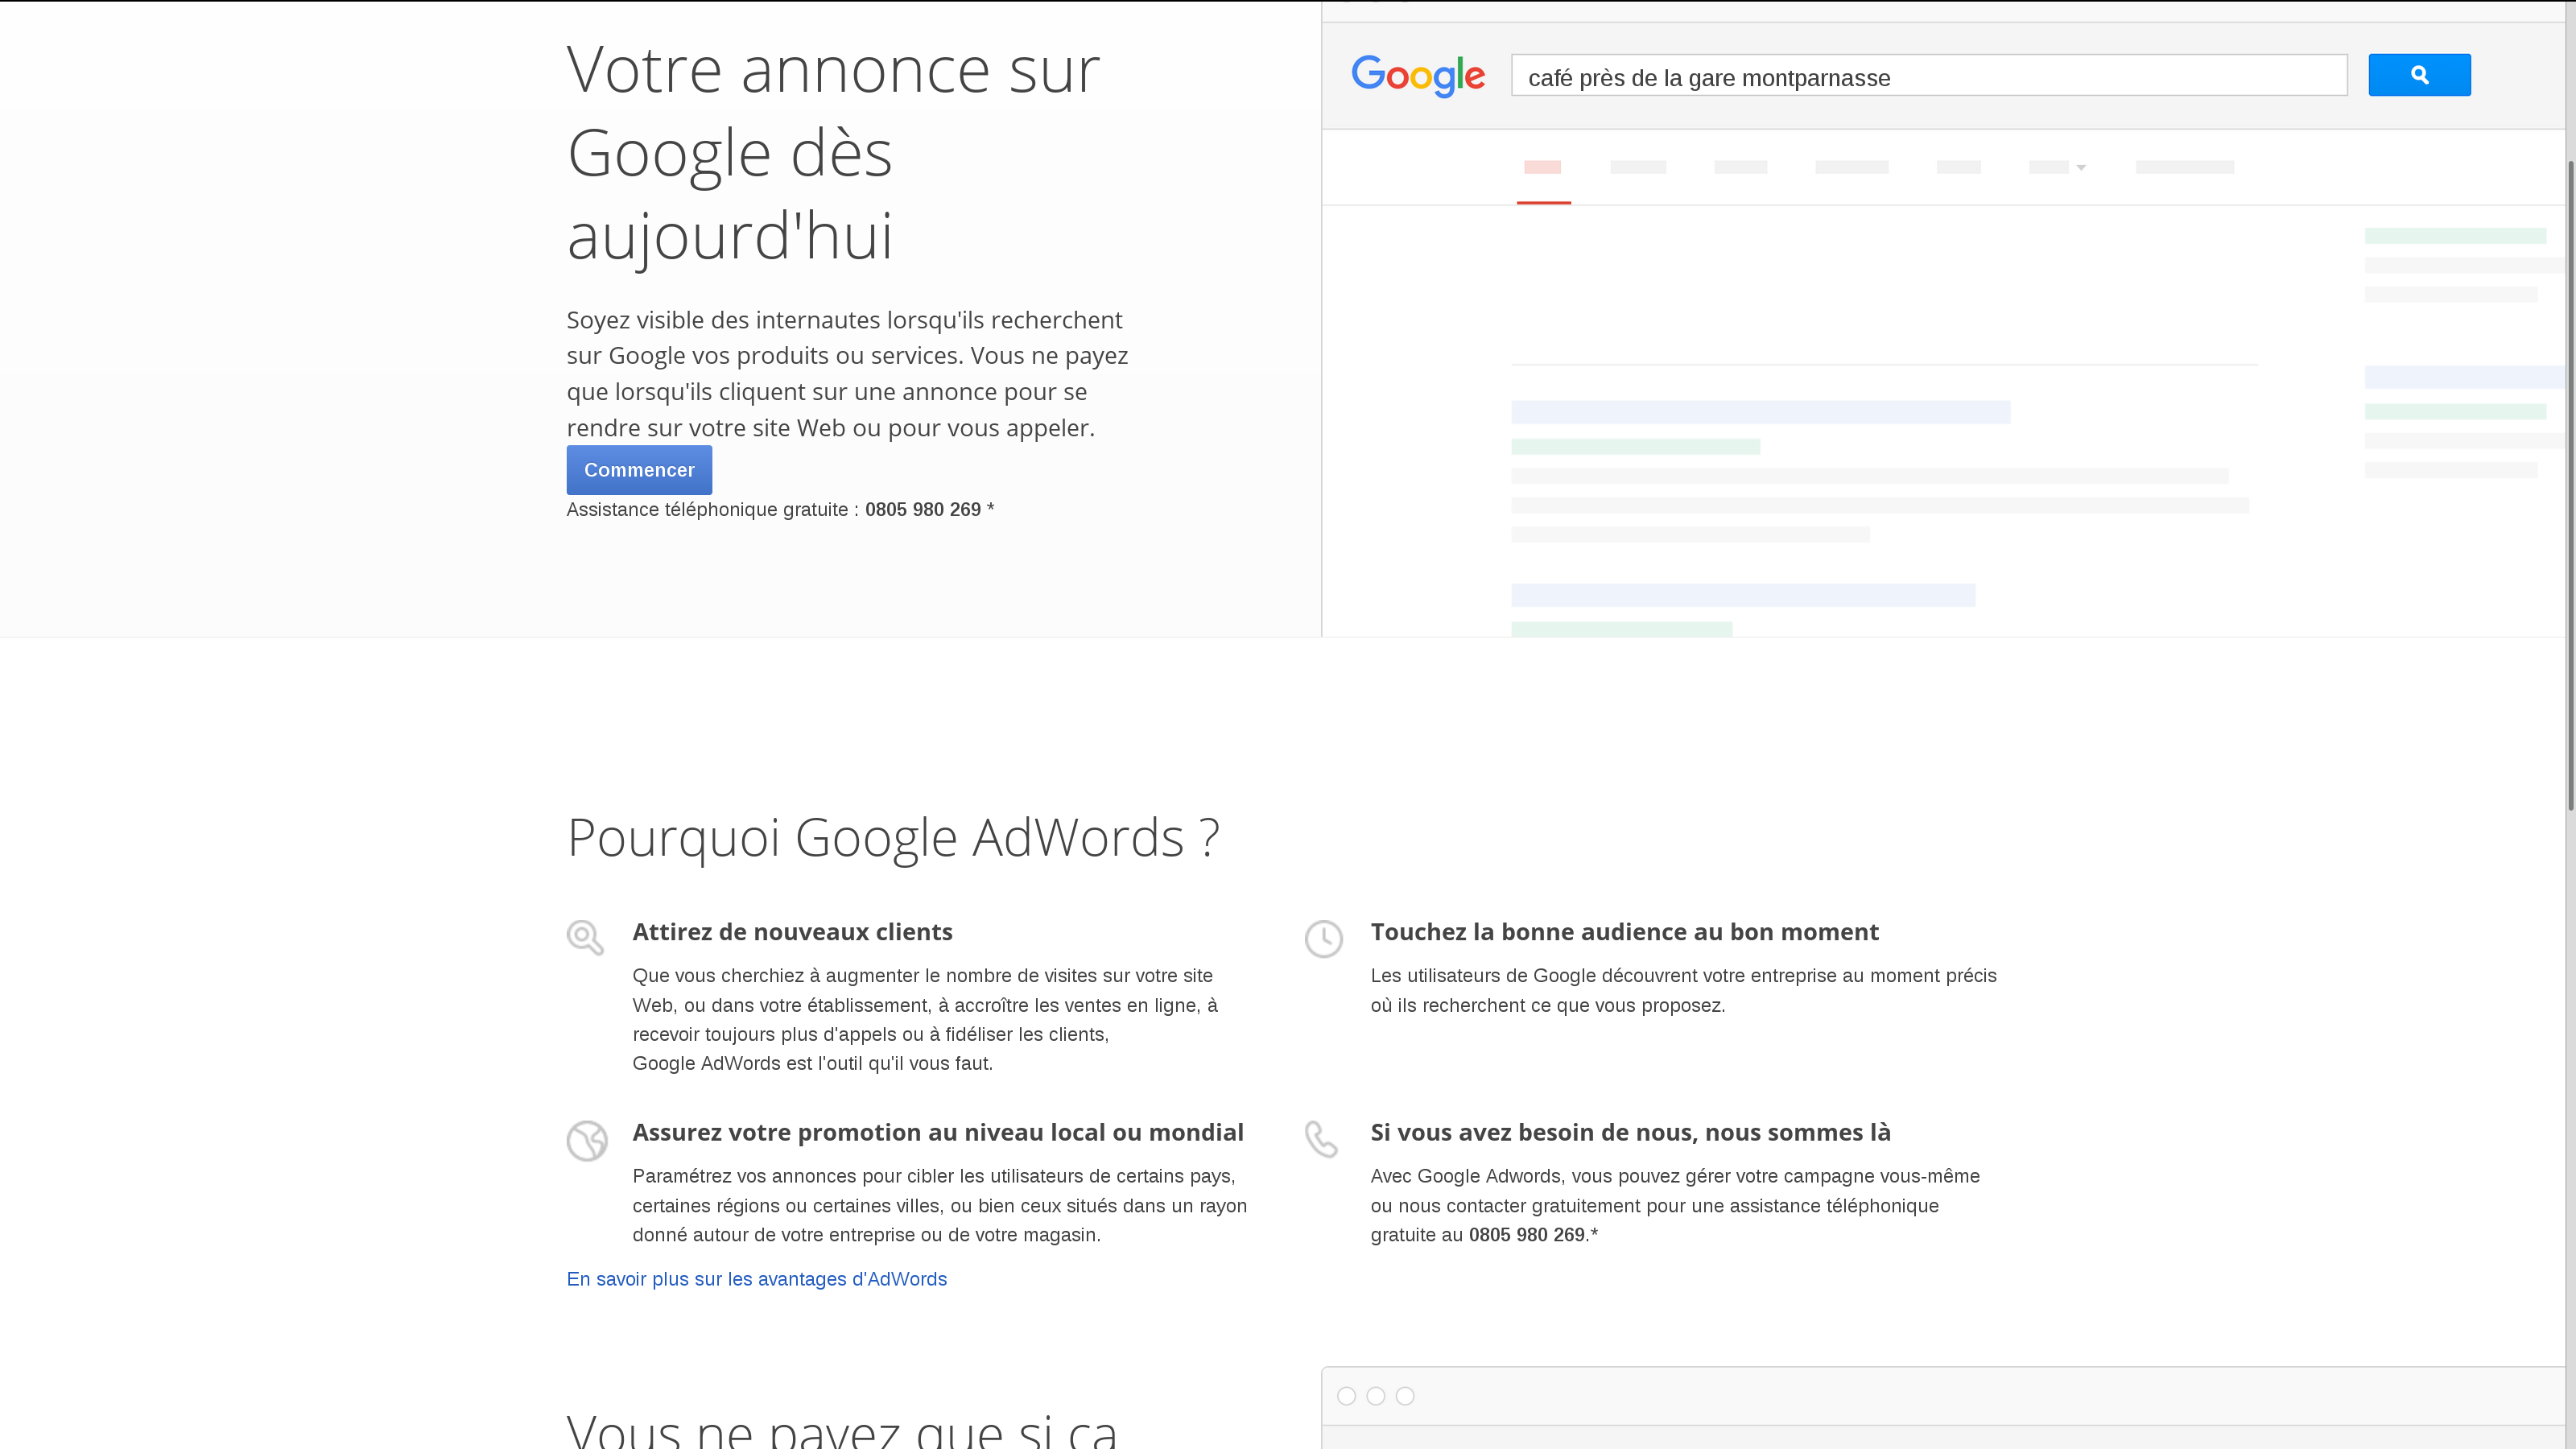
\includegraphics[width=\textwidth,height=\textheight,keepaspectratio]{./google.png} 
\end{frame}
}

\begin{frame}
{Gratuit, vraiment ?}
\begin{itemize}
\item Publicités insérées dans vos messages
\item Publicités insérées dans les résultats de recherches
\item Publicités insérées sur les sites visités
\item …
\end{itemize}
\centering
Et le tracking constant !
\end{frame}

\begin{frame}
{"Dans votre intérêt"}
\begin{itemize}
\item "Optimisations" des recherches
\item Assistant personnel (google now, etc)
\item …
\end{itemize}
\end{frame}

\begin{frame}
{Mais c'est pratique !}
\begin{itemize}
\item Ces "features" vous confortent dans le don de vos données
\item Au final, votre bénéfice est moindre par rapport à celui de ces sociétés
\end{itemize}
\end{frame}

\begin{frame}
{En résumé…}
\centering
\color{red}Si on ne vous vend rien, c'est VOUS que l'on vend !
\end{frame}

{
\hypersetup{
        colorlinks=true,
        linkcolor=white,
        urlcolor=white
}
\setbeamertemplate{headline} {
        \begin{beamercolorbox}[wd=\paperwidth,dp=8pt,ht=12pt,leftskip=.29cm,rightskip=.29cm]{linecolor}
        Source: \textbf{\href{http://spotfire.tibco.com/blog/?p=23638}{Tibco Spotfire}}
        \hfill
        \insertinstitute
        \end{beamercolorbox}%
}
\begin{frame}
\centering

\includegraphics[width=\textwidth,height=\textheight,keepaspectratio]{./money-cloud.jpg} 
\end{frame}
}

\begin{frame}
{Et l'Opensource dans tout ça ?}
\begin{itemize}
\item Aussi gratuit
\item Aussi des applications/services
\item Parfois de la publicité
\end{itemize}

\vspace{1cm}
\centering
¿! Quelle différence ?!
\end{frame}

\begin{frame}
{Tout est question de contrôle}
\begin{itemize}
\item Code source disponible
\item Communauté
\item Contacts avec les développeurs
\end{itemize}
\end{frame}

\begin{frame}
{L'Opensource à l'aide}
\begin{itemize}
\item Une bonne partie des solutions se trouvent dans l'Opensource
\item Des applications libres, ouvertes, pas forcément gratuites
\end{itemize}
\end{frame}

\begin{frame}
{Bullshit-o-mètre}
\begin{itemize}
\item Hébergé en Suisse
\item Chiffrement de grade militaire
\item Notre logiciel breveté
\item Notre algorithme révolutionnaire
\end{itemize}
\end{frame}

\begin{frame}
{Alternatives ouvertes au commercial fermé}
\begin{itemize}
\item Facebook : \href{https://diasporafoundation.org/}{Diaspora*}
\item Twitter : \href{http://twister.net.co/}{Twister}
\item GMail : plus compliqué, dépend des besoins
\item DropBox : \href{https://owncloud.org/}{OwnCloud}, \href{https://www.seafile.com/en/home/}{Seafile}
\end{itemize}
\end{frame}

\begin{frame}
{Les sites à connaître}
\begin{itemize}
\item \href{https://prism-break.org/en/}{Prism Break}
\item \href{http://degooglisons-internet.org/}{Dégooglisons Internet}
\end{itemize}
\end{frame}

\begin{frame}
{Les hackerspaces sont là pour aider}
\centering
\href{https://wiki.hackerspaces.org/}{Trouver un hackerspace}

\vspace{1cm}
À Lausanne : \href{https://fixme.ch/}{Fixme}
\end{frame}

\begin{frame}
{Cryptoparties}
Les cryptoparties permettent à tout le monde de comprendre et d’acquérir les compétences.

\vspace{0.5cm}
\centering
\href{https://www.cryptoparty.in/}{Plus d'informations}

\vspace{1cm}
À Fribourg : \href{https://cryptofribourg.ch/}{CryptoFribourg}
\end{frame}

\begin{frame}
{Exemple comparatif}
\center
Signal vs WhatsApp
\end{frame}

\begin{frame}
{Whatsapp}
\begin{itemize}
\item Gratuit (de nouveau)
\item Code fermé
\item Aucun contrôle communautaire
\item Facebook :)
\item Modèle économique vaseux
\end{itemize}
"the company hopes “to work with businesses and organizations you want to hear from.”" \newline

\href{http://uproxx.com/webculture/now-free-again-heres-how-whatsapp-plans-to-make-money-with-no-ads/}{Source}
\end{frame}

\begin{frame}
{Signal}
\begin{itemize}
\item Gratuit
\item Code ouvert
\item Contrôle communautaire
\item Indépendant
\item Chiffrement vérifiable
\end{itemize}
\end{frame}


\begin{frame}
{Tout n'est donc pas perdu !}
\begin{itemize}
\item En employant vous-même des alternatives
\item En parlant des alternatives autour de vous
\item En partageant vos expériences
\item En rapportant des bugs aux développeurs
\end{itemize}
\end{frame}

{
\setbeamertemplate{footline}{%
	\begin{beamercolorbox}[wd=\paperwidth,dp=8pt,ht=12pt,leftskip=.29cm,rightskip=.3cm]{linecolor}
	\hfill
	\inserttitle
	\end{beamercolorbox}%
}
{
\centering
\begin{frame}
{Questions ?}

\href{https://ethack.org/}{https://ethack.org/} \\
\vspace{0.3cm}
\href{https://www.twitter.com/EthACK_org}{@EthACK\_org} on Twitter \\
\vspace{0.3cm}
\href{https://www.facebook.com/ethack.org}{ethack.org} on Facebook

\vspace{0.5cm}


\includegraphics[width=4cm]{../common/logo_537.png}
\end{frame}
}
}

\end{document}